\section{Description and event displays of high $\etmiss$ events}

\subsection{EB, spike at EB-EE boundary}
We see EB spikes occurring at the boundary between ECAL barrel and endcaps.

The ECAL spikes topological cuts employed in the calotower cleaning for Calo$\etmiss$ and tc$\etmiss$ 
are not currently applied to identify ``spikes'' candidates occuring at the boundary between ECAL barrel and endcaps. 
Most of such events should be removed by the timing cuts. Nevertheless, some of them still survives 
after the noise clean-up, as the event shown in Figure~\ref{fig:EBspikeAtBorder}.

Such EB spikes are instead all cleaned by PF cleaning, which applies relaxed topological cuts also at the EB-EE boundary.
%
\begin{figure}[h]
 \centering
% \begin{tabular}{ll}
   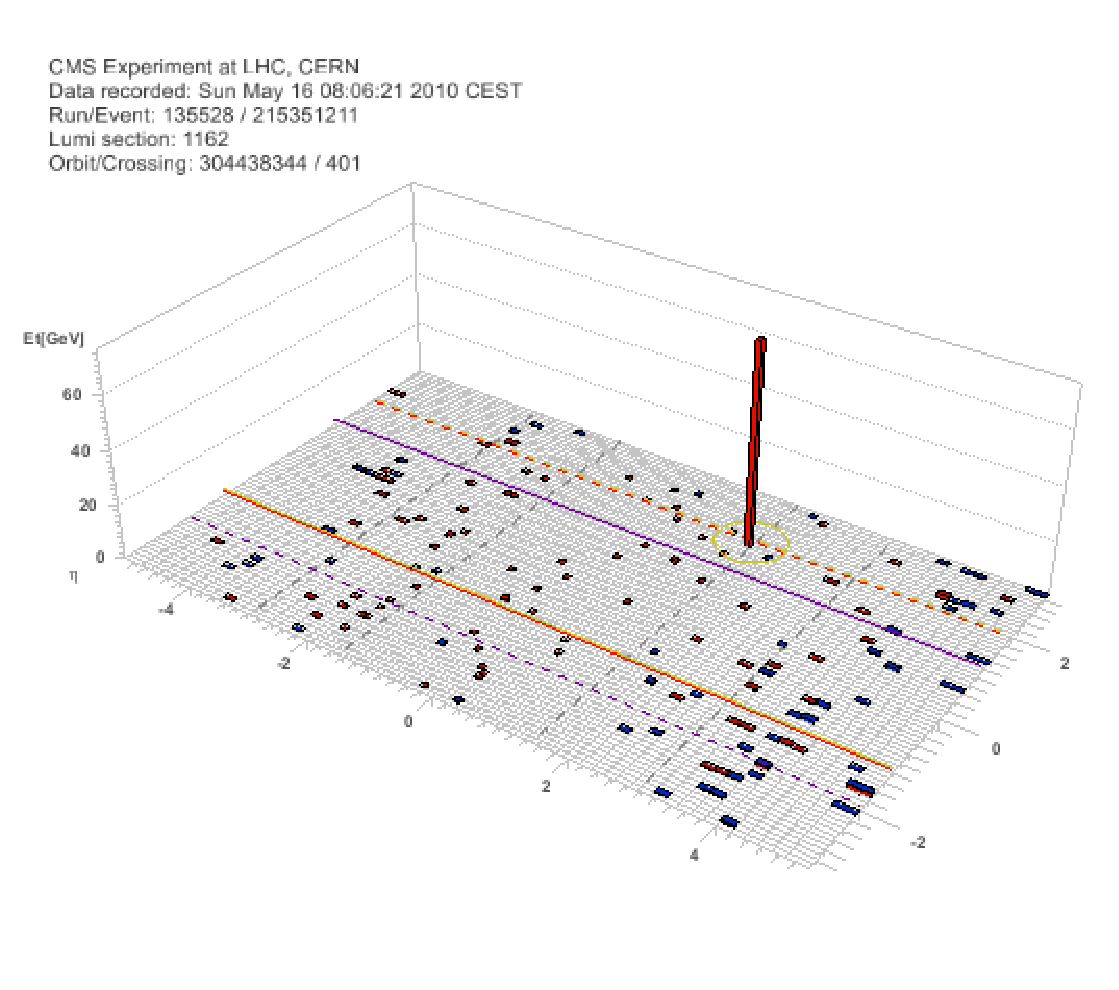
\includegraphics[width=0.47\textwidth]{fig/EBspikeAtBorder.eps} 
% \end{tabular}
\caption{Example of ``EB spike at EB-EE boundary'' event}
\label{fig:EBspikeAtBorder}
\end{figure}

\subsection{EB, EE spikes}
We see one event with an isolated spike in EB (Figure~\ref{fig:EBEEspike}, left plot) 
and one event with an isolated spike in EE (Figure~\ref{fig:EBEEspike}, right plot), both far from the EB-EE boundaries.

Calotower-based cleaning for spikes is not applied in EE (since the spikes has been observed and understood 
as due to interaction of particles in APD, which are mounted only in the barrel). 
The case of EB spike not cleaned should be investigated.

Both events are cleaned by PF (which applies spike cleaning also in EE).
%
\begin{figure}[h]
 \centering
 \begin{tabular}{ll}
   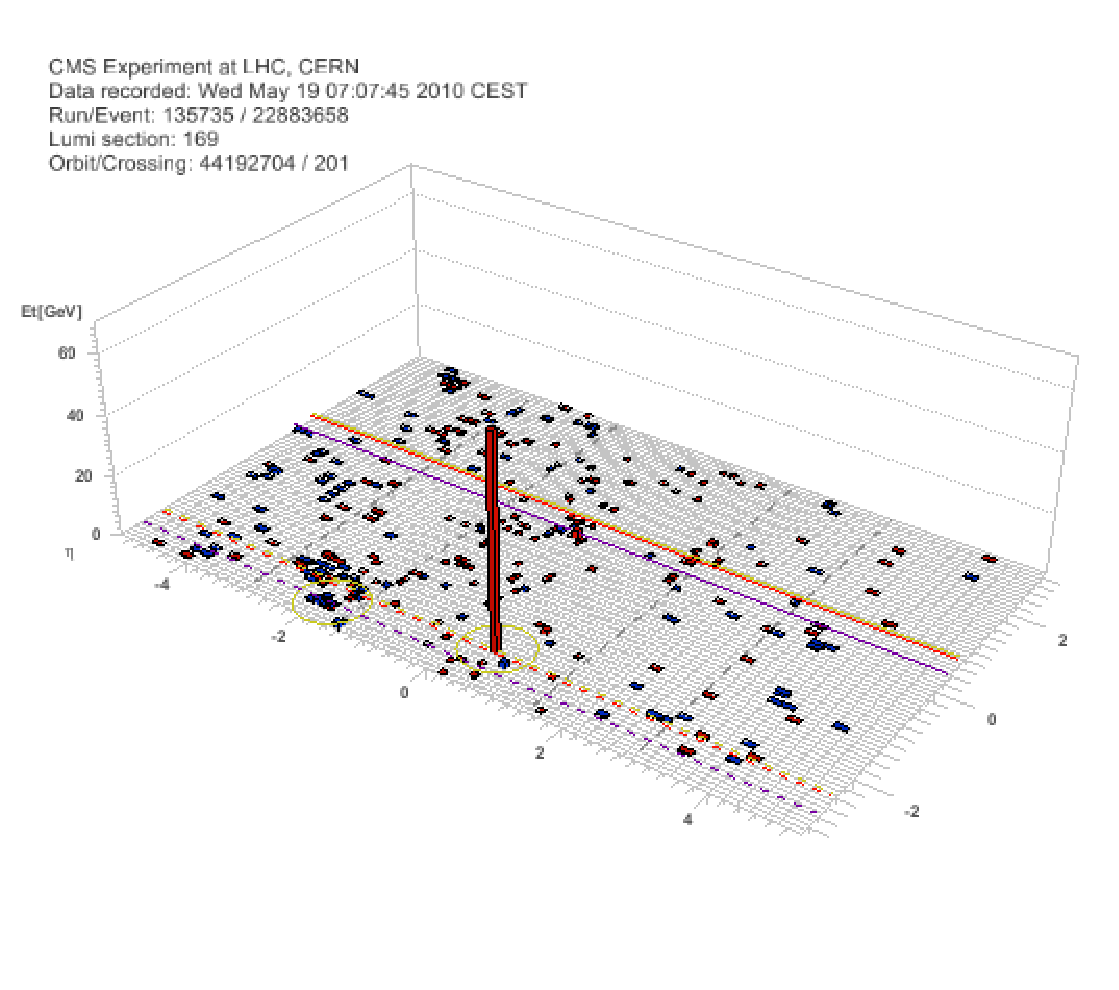
\includegraphics[width=0.47\textwidth]{fig/EBspike.eps} &
   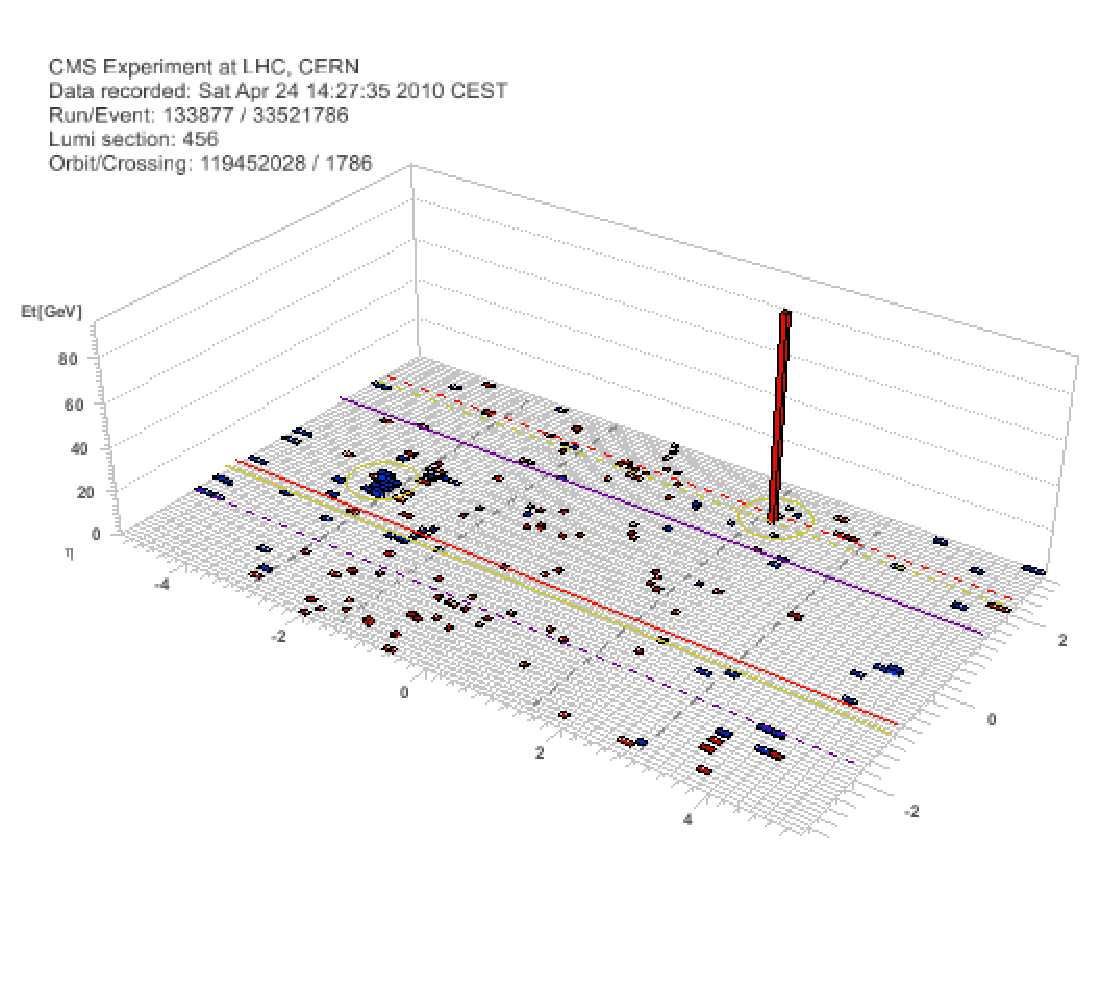
\includegraphics[width=0.47\textwidth]{fig/EEspike.eps} \\
 \end{tabular}
\caption{Example of EB spike (left) and EE spike (right) event}
\label{fig:EBEEspike}
\end{figure}


\subsection{HF, multi-PMT-hits or phi-strip events}
These events are characterized by several PMT hits in adjecent cells; sometimes they show up as
a strip of hits at the same $i\phi$ location, as the ones reported in Figure~\ref{fig:HFmultiHits}. 
This type of noise cannot be cleaned by the existing topological algorithms but could 
be cleaned by the timing or pulse shape based 
cleaning if hits are out-of-time or have a malformed pulse shape. 
A topological cleaning based on the multiplicity of hits above certain energy threshold 
at the same $i\phi$ location might be effective at identifying such noise.
The source of such events is not yet fully understood.

Some of these events are identified by PF cleaning but not by calotower based cleaning.
Studies are ongoing to understand the differences.

%
\begin{figure}[h]
 \centering
 \begin{tabular}{ll}
   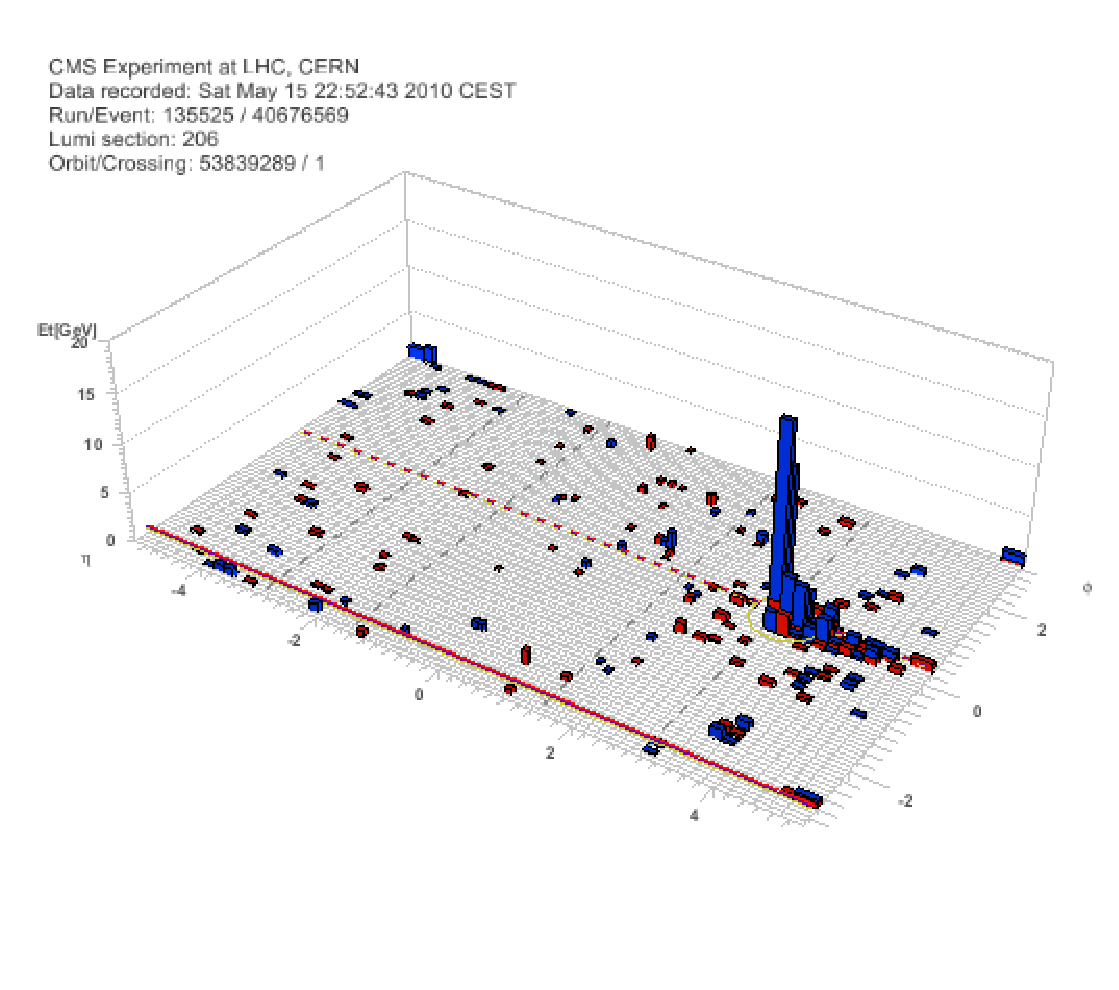
\includegraphics[width=0.47\textwidth]{fig/HFmultiHits.eps} &
   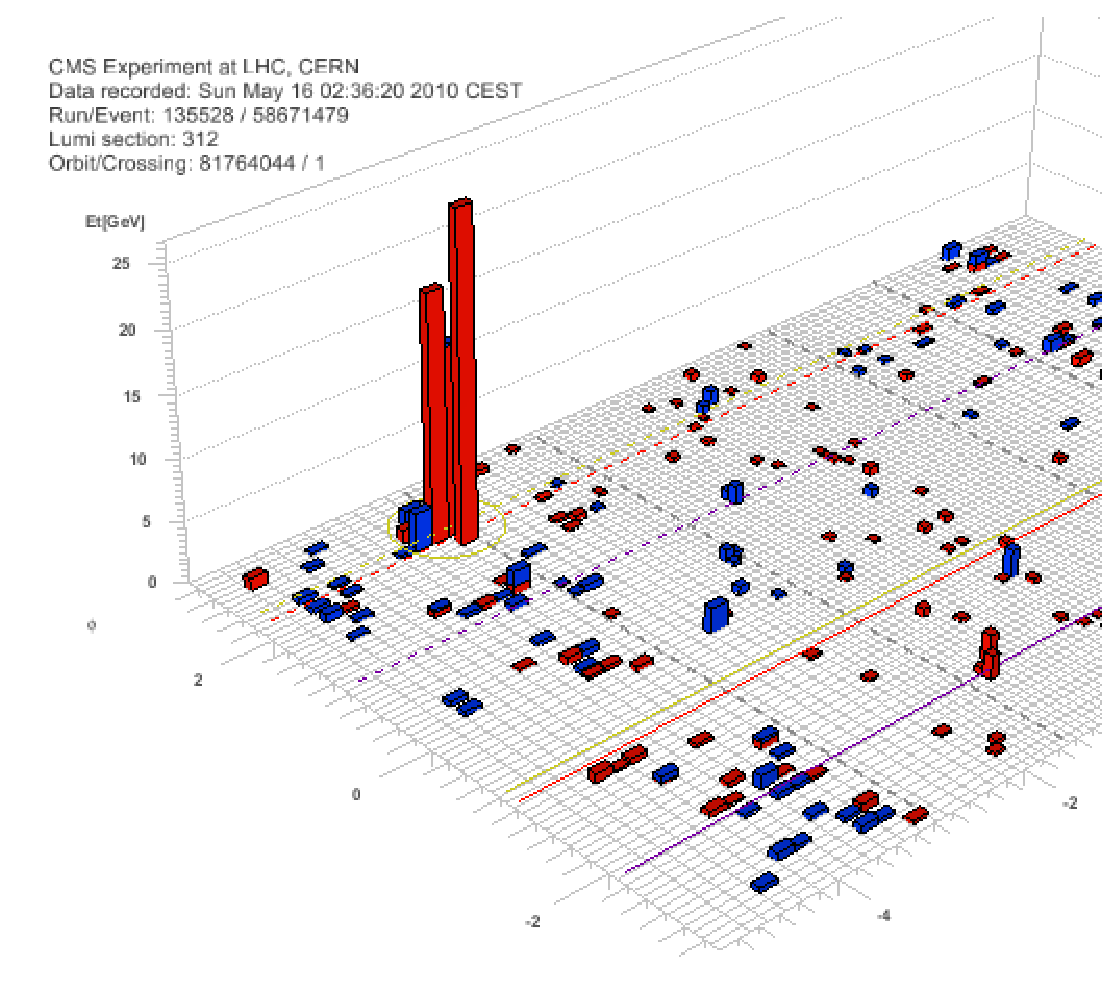
\includegraphics[width=0.47\textwidth]{fig/HFmultiHits_2.eps} \\
 \end{tabular}
\caption{Example of two ``HF multi-PMT-hits or phi-strip'' events}
\label{fig:HFmultiHits}
\end{figure}

\subsection{HF, double-PMT-hits}
These events are characterized by significant energy in both long and short fibers in a single
isolated tower, as shown in Figure~\ref{fig:HFdoublehits}. For high $\etmiss$ events, 
this noise often shows up in the towers located at the smallest $\eta$ 
value in HF ($\eta$=3). This can be explained by the fact that, for a given energy, 
a noise occurring at smaller $\eta$ produces a larger transverse energy, and therefore is more visible at high $\etmiss$.
Anyway it's not excluded that double-hits occurrs also at larger $\eta$; but in this case such events might 
fall in the bulk of $\etmiss$ distribution.

This type of noise cannot be cleaned by current calotower-based topological algorithms (PET or S9/S1) but can
be cleaned by the timing or pulse shape based cleaning if hits are out-of-time or have a malformed pulse shape.
However, cases of in-time double-hits with good pulse shape have been observed. In such cases, a cleaning based on
S$8$/S$1$ isolation variable could be effective, where S$8$/S$1$ is defined in a similar way to S$9$/S$1$
with the companion RecHit energy from the same HF tower left out from the sum. 
On the other hand, this type of cleaning is not expected to be fully safe for isolated particles, 
in particular for physically bigger towers at lower $\eta$ values. 
Preliminary studies on the use of S$8$/S$1$ isolation variable have been performed but not yet finalized. 

PF cleaning can flag some of these noisy events. Studies are ongoing to understand the differences.

%
\begin{figure}[h]
 \centering
 \begin{tabular}{ll}
   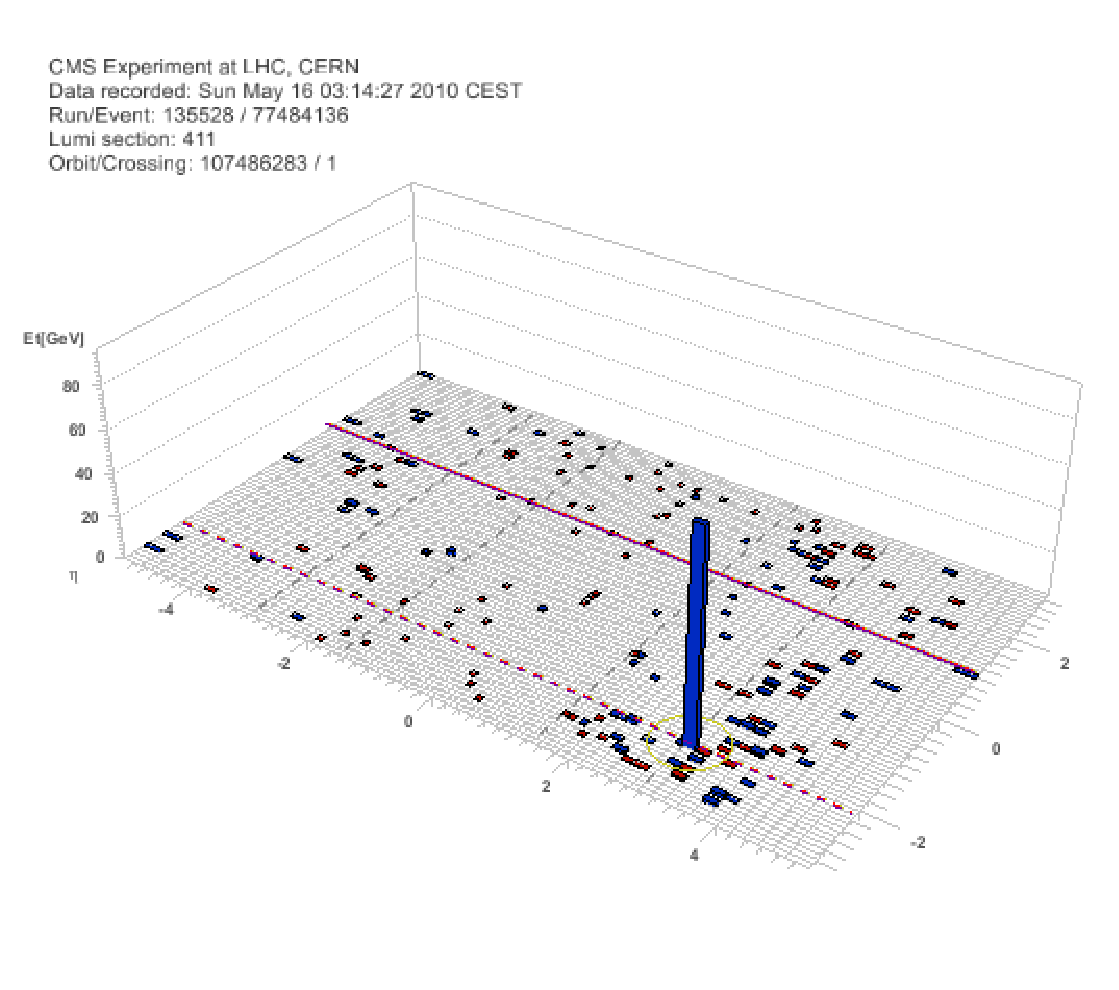
\includegraphics[width=0.47\textwidth]{fig/HFdoubleHit.eps} &
   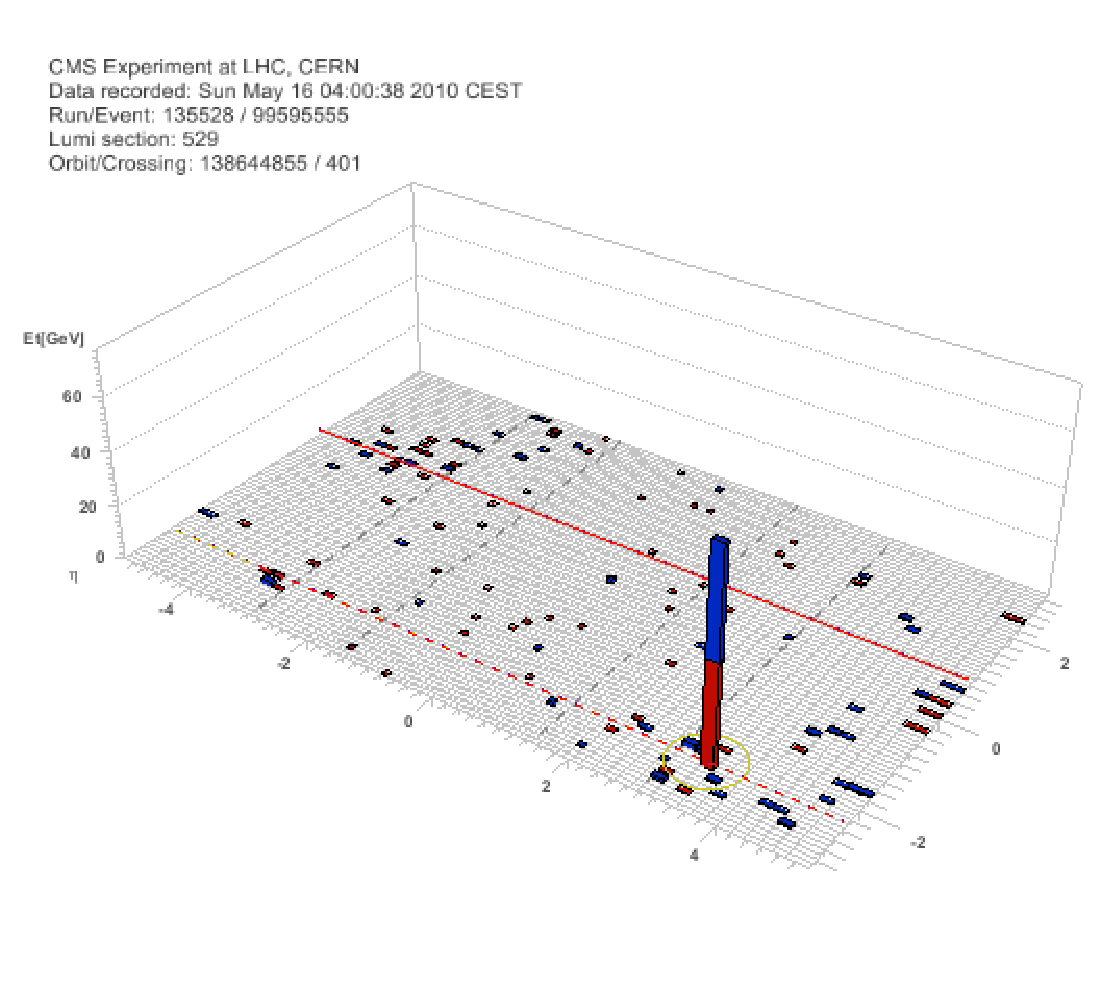
\includegraphics[width=0.47\textwidth]{fig/HFdoubleHit_1.eps} \\
 \end{tabular}
\caption{Example of ``HF double-PMT-hits'' events. Event in left plot is cleaned by PF and not by 
calotower-based cleaning; the event on the right is not cleaned by any of the two. 
NOTE: The event display for the left plot is mis-leading since the hit is not single, 
as it would seems, but double. In fact, in HF, blue=2*$E_{S}$=hadEnergy, while red=$E_{L}-E_{S}$=emEnergy. 
In this event the emEnergy (``red'') is negative, but both energies in long and short fibers, $E_{L}$ and $E_{S}$, are large
(several undreds of GeV). The event display only shows positive quantities 
(only the hadEnergy = ``blue'') so the negative ``red'' is not visible and gives the illusion of a single hit. 
Most of events cleaned by PF have negative emEnergy.}
\label{fig:HFdoublehits}
\end{figure}

\subsection{HF, PMT hit embedded in a jet} ~\label{sec:HFHitEmbeddedInJet}
These events are characterized by one or more anomalous hits embedded inside a jet,as shown in 
Figure~\ref{fig:HFhitEmbeddedInJet}. This type of noise could arise from muons coming from 
in-flight decays of hadronic particles or from a jet punch-through. In both cases
such jets could be identified using the JetID variables since it is expected that a large fraction of the
total jet energy would come from only one or two HF towers. Due to an overlap between real and anomalous signal there are
two cleaning strategies possible: an entire event could be rejected or a more sophisticated anomalous energy
subtraction algorithm would have to be developed.
%
\begin{figure}[h]
 \centering
 \begin{tabular}{ll}
   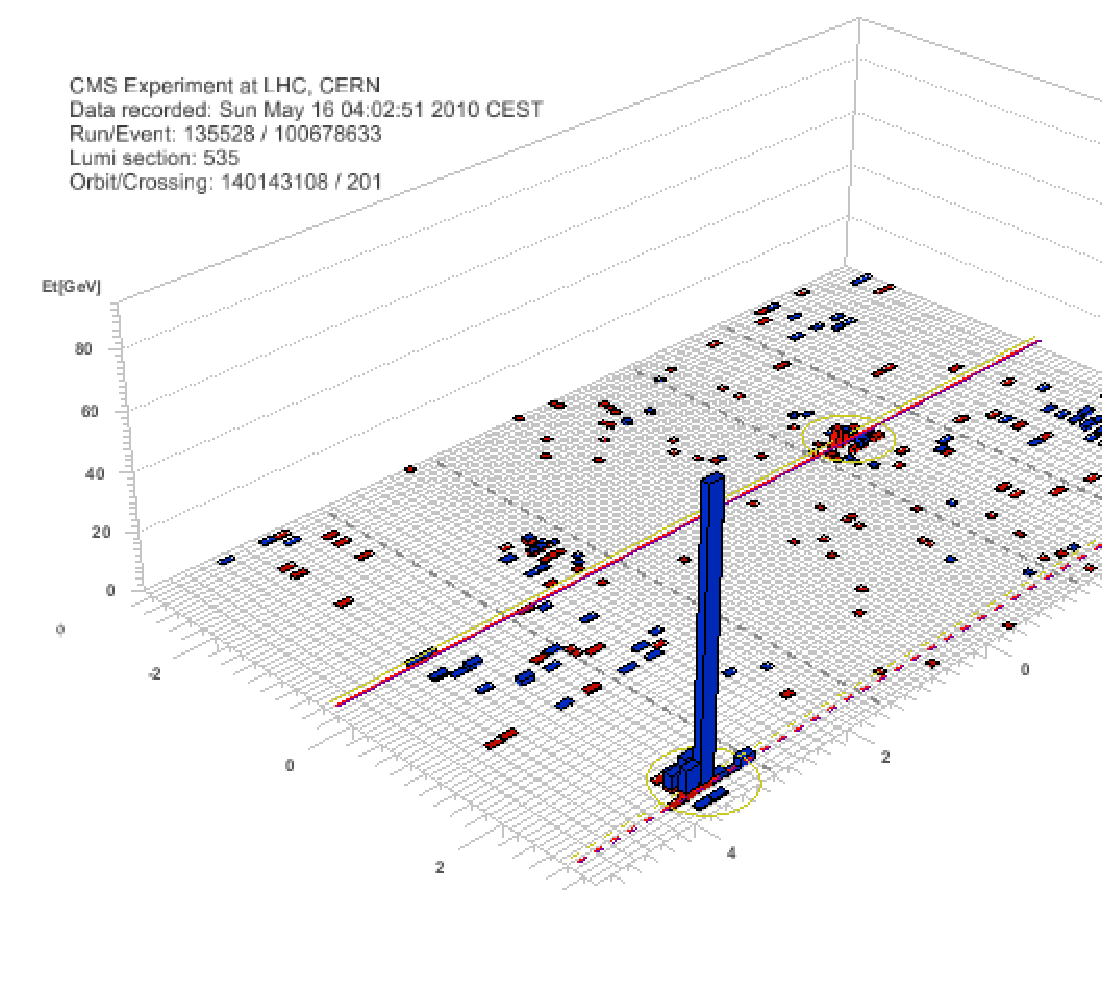
\includegraphics[width=0.47\textwidth]{fig//HFhitInJet.eps} & 
   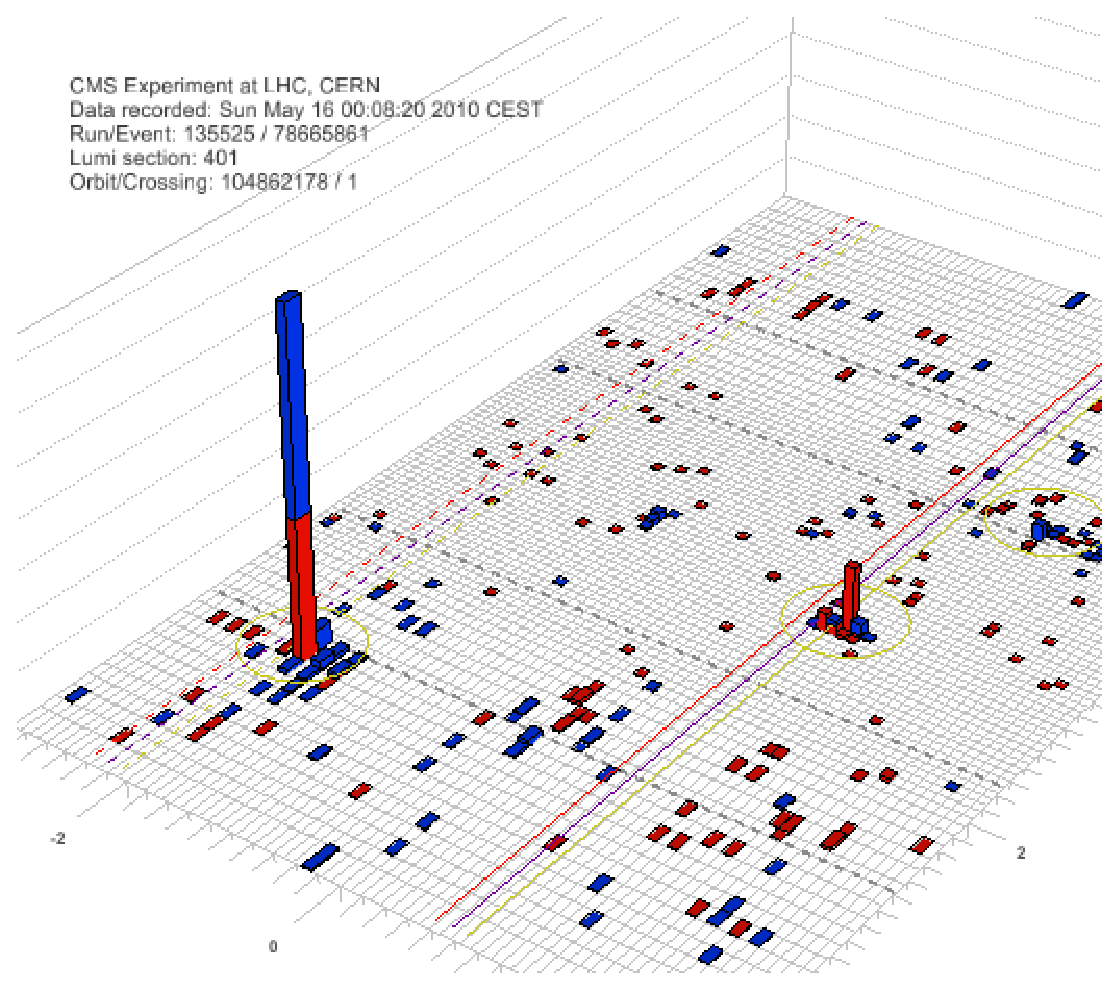
\includegraphics[width=0.47\textwidth]{fig//HFhitInJet_1.eps} \\
 \end{tabular}
\caption{Example of ``HF PMT hit embedded in a jet'' events}
\label{fig:HFhitEmbeddedInJet}
\end{figure}

